\documentclass{amsart}

\usepackage{graphicx}
\usepackage{textcomp}
\usepackage{amsmath}
\usepackage{amsthm}

\newtheorem{theorem}{Theorem}[section]

\renewcommand{\vec}{\textbf}

\theoremstyle{definition}
\newtheorem{definition}{Definition}

\title{Projectile Motion on a Space Station}

\begin{document}
\begin{abstract}
 Something
\end{abstract}
\maketitle


\section{Gravity via centripetal acceleration}


In science fiction, artificial gravity for space-craft and
space-stations is often generated via centripetal acceleration, see
\cite{2001,2010,missiontomars,themartian,expanse,babylon5,europareport,ringworld?,rama,intersetller,etc}
for an incomplete list. Usually characters live inside a cylinder that
is spinning, such as the von Braun Wheel depicted in figure
\ref{fig:Braun Wheel}.

\begin{figure}[h]
  \centering
  \includegraphics[width=0.5\textwidth]{Von_Braun_1952_Space_Station.jpg}
  %wikipedia von Braun Wheel
  \caption{von Braun Wheel}
  \label{fig:Braun Wheel}
\end{figure}

Centripetal acceleration pushes them against the outside wall of the
cylinder. In television and film, (surely due to production
limitations) this ``artificial gravity'' is portrayed as being an
excellent facsimile for Earth's gravity. In this paper we seek to
answer the question of how accurately centripetal acceleration mimics
gravitational acceleration.


% Papers that did similar things to ours
% http://davidkann.blogspot.com/2014/06/oneill-cylinder-simulator-projectile.html (Build a simulator)
% https://kaiserscience.wordpress.com/physics/rotational-motion/artificial-gravity-in-a-space-station/



While centripetal acceleration (on cylindrical space-craft etc.) has
been extensively studied \cite{papers,anotherpaper}, most of these
studies focus on the fictitious forces present on a space stateion and
the basic consiquences these have on the equations for projectile
motion. In this paper we seek to expand on these papers and flush out projectile motion on
spaceship with centripital acceleration. Ultimately we should become
comfortable with projectile motion and we should provide some basic
answers to questions like: What is the maximum height of a projectile?
At what point does a projectile ``loop'' around? How might one play a
game of catch on a ship with centripital acceleration?

\subsection{Projectile Motion from Ring World Inhabitant Perspective}


When on a planet where the acceleration due to gravity is $g$, we know
that an object thrown at an angle of $\theta$ from the horizontal at
an initial speed of $v_0$, with an initial position of $(x_0,y_0)$
follows the path of:
\begin{align*}
  x_{\mathrm{planet}}(t) &=  v_0 t \cos(\theta)  + x_0\\
  y_{\mathrm{planet}}(t) &=  -g/2 t^2 + v_0 t \sin(\theta)  + y_0
\end{align*}
These equations of projectile motion describe the path an object takes
after being thrown.

%Generic gravity Projectile motion plot
\begin{figure}[h]
  \centering
  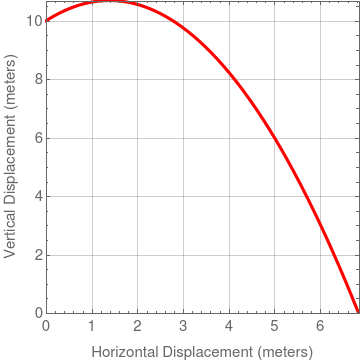
\includegraphics[width=0.5\textwidth]{Projectile_In_Gravity.png}
  \caption{Projectile thrown in standard gravity takes the path of a parabola.}
  \label{fig:Braun Wheel}
\end{figure}

We seek analogous equations that show the path of a projectile on a
rotating space station. In particular, we wish to show the path from
the view-point of people on the station.  From this perspective,
\textit{vertical} is defined as the distance from the floor of the
habitation ring and \textit{horizontal} is defined as the arc length
counter clockwise or clockwise from the observer.

[[image]]


Thus the equations of motion for a projectile ((seems a bit quick!))
from the Ring World Inhabitant Perspective are:

\begin{align*}
  p_{r}(t) &= t^2 (v_x + \omega r_0 Cos(\omega t_0))^2 + (t(v_y + \omega
  r_0 Sin(\omega t_0) - R))^2\\
  p_{\theta R}(t) &=R ArcTan(t(V_x + \omega r_0 Cos(\omega t_0)),tV_y +
                    t \omega r_0 Sin(\omega t_0))
\end{align*}

\begin{figure}[h]
  \centering
  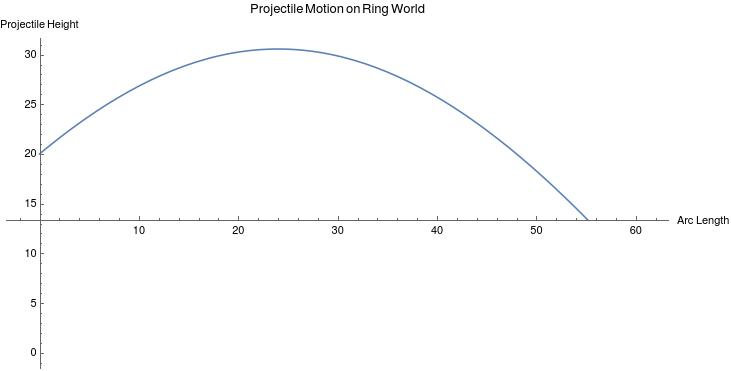
\includegraphics[width=0.7\textwidth]{ArclengthProjectileLabeled.jpg}
  \label{fig:shipview}
  \caption{}
\end{figure}


\begin{figure}[h]
  \centering
  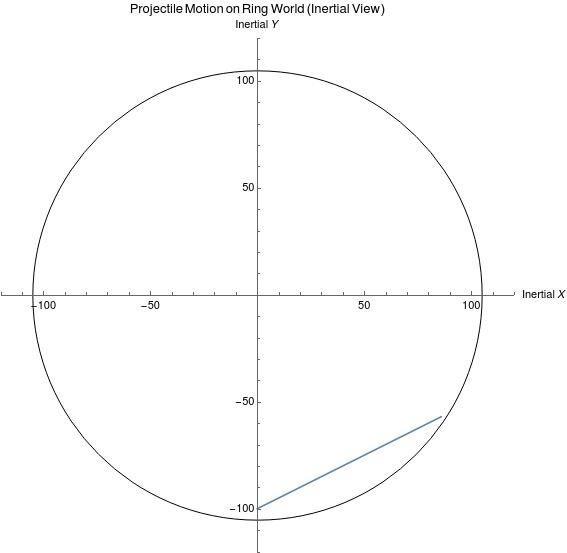
\includegraphics[width=0.7\textwidth]{InertialArclengthProjectileLabeled.jpg}
  \label{fig:inertialview}
  \caption{}
\end{figure}

Figure \ref{fig:shipview} depicts projectile motion (a ball thrown at
45 degrees) using the Ring World equations of motion above. Note that
figure \ref{fig:inertialview} depicts the same throw event in figure
\ref{fig:inertialview}, except from the outside inertial
perspective. Something interesting to note is that from the outside
perspective,the ball is not being thrown at a 45 degree angle with
respect to the thrower's horizontal axis (I wonder why that is).


\section{Acrobatics}



\begin{theorem}
  Given a space station of radius $r$ and angluar velocity $\omega$, the maximum height that can be thrown with realistic behavior is....
\end{theorem}





Suppose an inhabitant of height $h$ decides to water their garden. The flowers are of arclength $R\Delta\Theta$ away. 

In order to find out, we will need to solve for the equations of
motion for free falling objects in Miller's frame. In particular we
will consider the case of a dropped ball. The most challenging aspect
of solving for the equations of motion in Miller's frame will be
determining the frame itself. As you'll see, defining up, down, left
and right on a spinning spaceship can be quite dizzying (pun
intended). We will approach the problem in two different ways. The
first method will take the viewpoint of an outside onlooker and use
rotation of frames to determine how the ball will fall from Miller's
perspective. In the second way, we will use the arclength of the ship
to describe the $x$ direction, while the distance from the ball to the
center of the ship, minus the ship radius itself describes the height
of the ball.

\subsection*{Method 1: Rotation of Frames}

From the view of the onlooker, Miller simply rotates around the ship at some angular velocity $\omega$ from a starting angle of $\phi$ from the vertical and the radius of the ship is $R$, Miller's position can be given by:

\begin{equation}\label{eq:MillerPosition}
    \vec{m}=R\cdot \langle cos(\theta(t)),sin(\theta (t)\rangle
\end{equation}

Where $\theta (t)$ is given by:

$$\theta (t) = \omega t$$
\[
    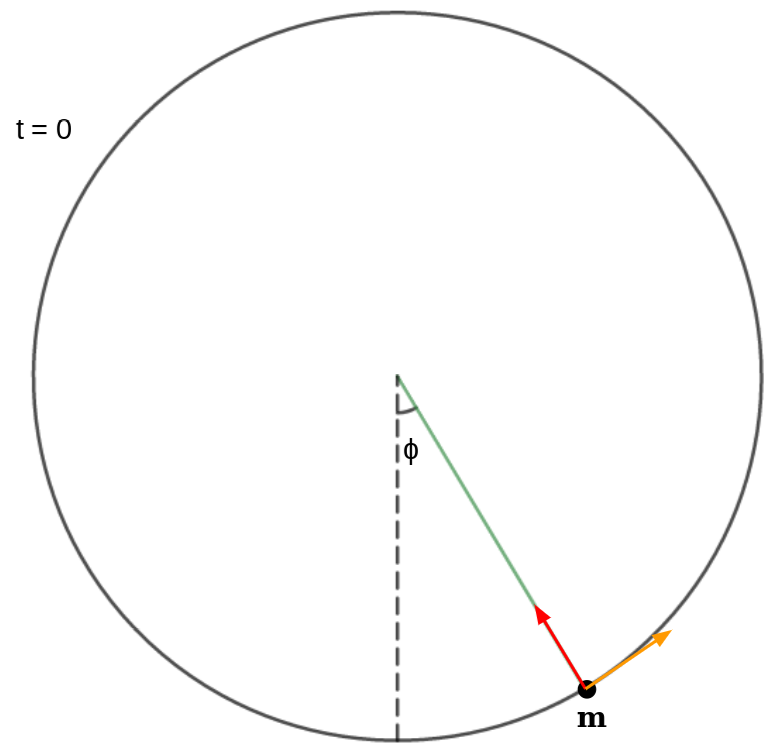
\includegraphics[width=.5\linewidth]{MillerZero.png}
    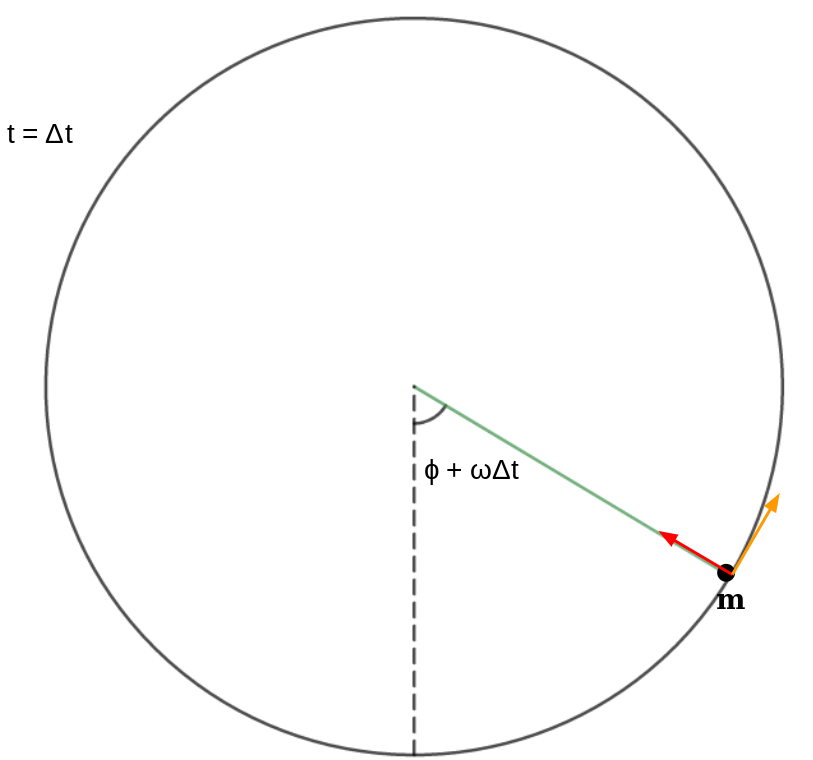
\includegraphics[width=.5\linewidth]{MillerDeltaT.png}
\]

Meanwhile the ball starts out at some point on the ship: $$\vec{b} = \langle x_0,y_0\rangle $$ moving with an initial velocity:

\[\vec{v}_0 = \vec{b}' = \frac{\omega}{2\pi} \langle -y_0,x_0\rangle\]

 where $\omega$ is considered positive when rotating counterclockwise.
    \[
    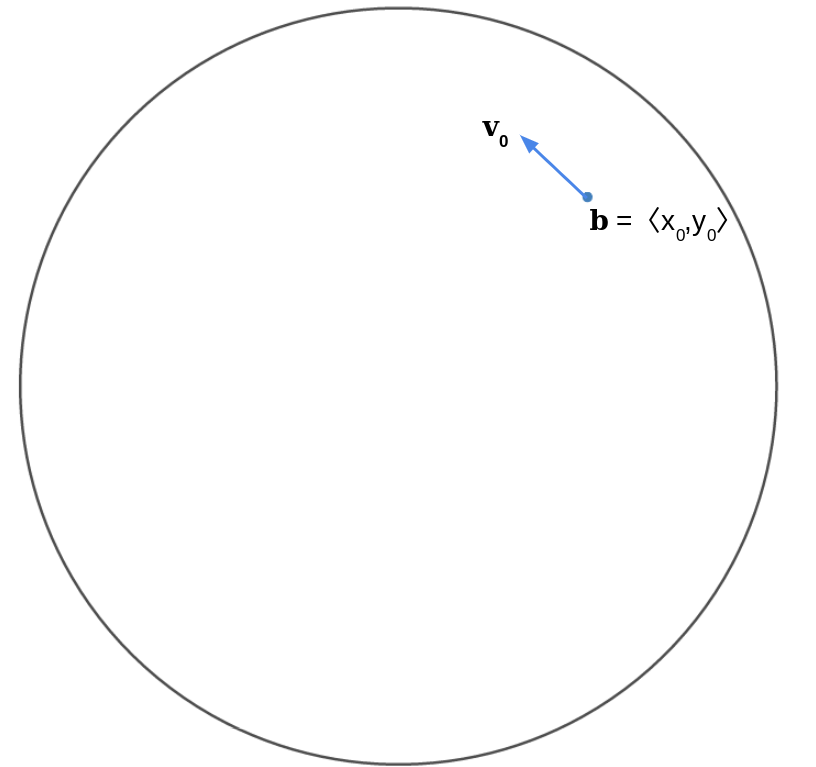
\includegraphics[natwidth = 300]{WaterInitial.png}
    \]
 Thus the paths that the onlooker will see for Miller and the ball are
\begin{equation}
\vec{m}=R\langle \sin(\theta(t)),-\cos(\theta (t)\rangle
\end{equation}

\begin{equation}\label{eq:BallV1}
\vec{b} = \langle x_0 - y_0 \omega t, y_0 + x_0 \omega t \rangle
\end{equation}

\[
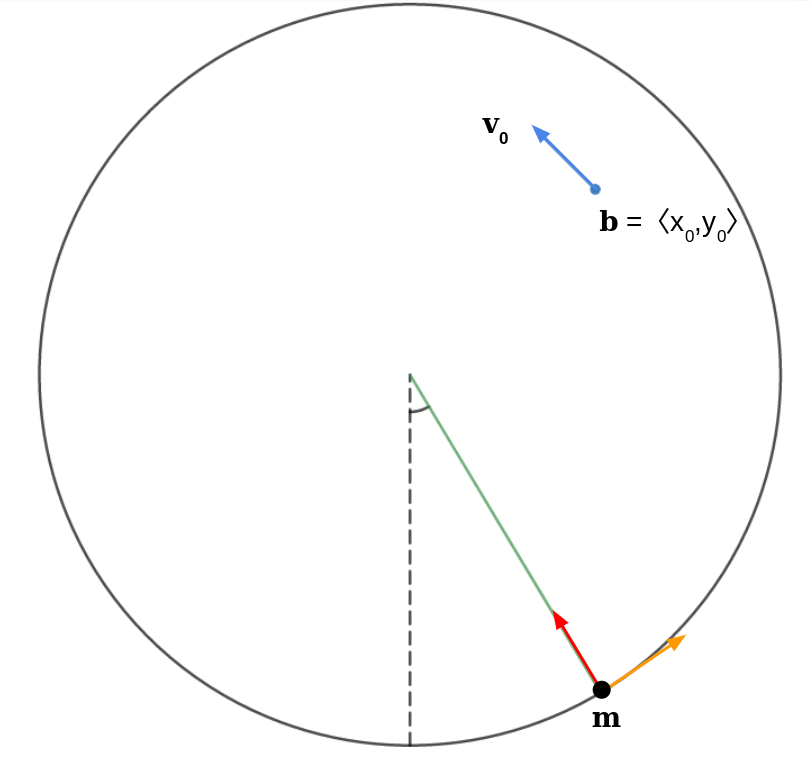
\includegraphics[natwidth = 300]{MillerAndWater.png}
\]

Now we want to draw a vector from Miller to the ball to find the ball's relative position to Miller. This is just a matter of subtracting Miller's position from the ball's position. We will call this vector $\vec{u}$ where:

\begin{equation}
    \vec{u}=\vec{b}-\vec{m}
\end{equation}

\[
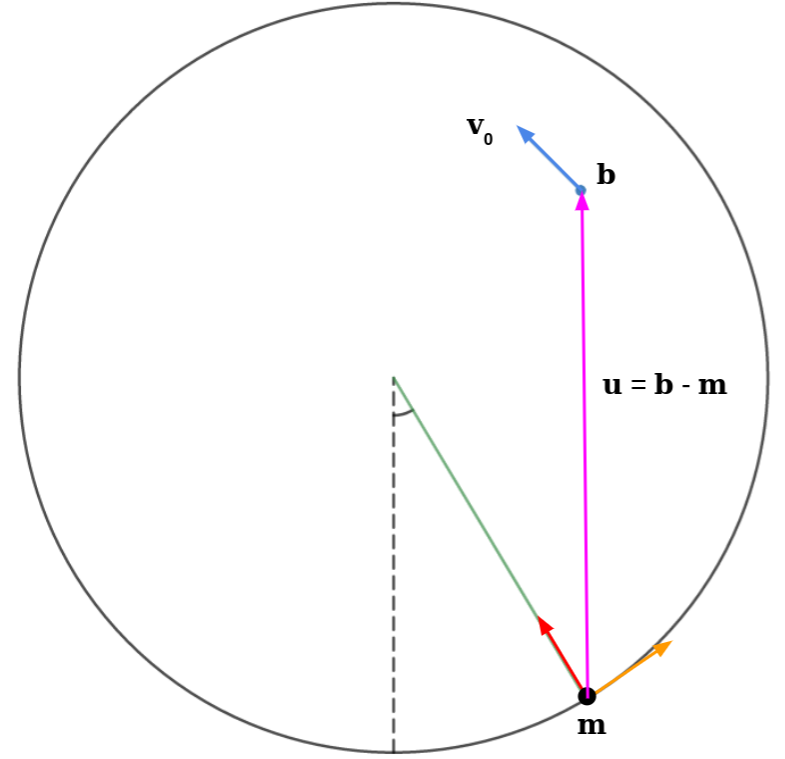
\includegraphics[width=.7\linewidth]{MillerWaterU.png}
\]

As shown above, \vec{u} points from Miller to the ball, which is exactly what we want! The only issue is that the vector is still in the eyes of the observer. While the observer has been sitting still in space, Miller's definition of $x$ and $y$ direction has been constantly changing from the observer's perspective.

\[
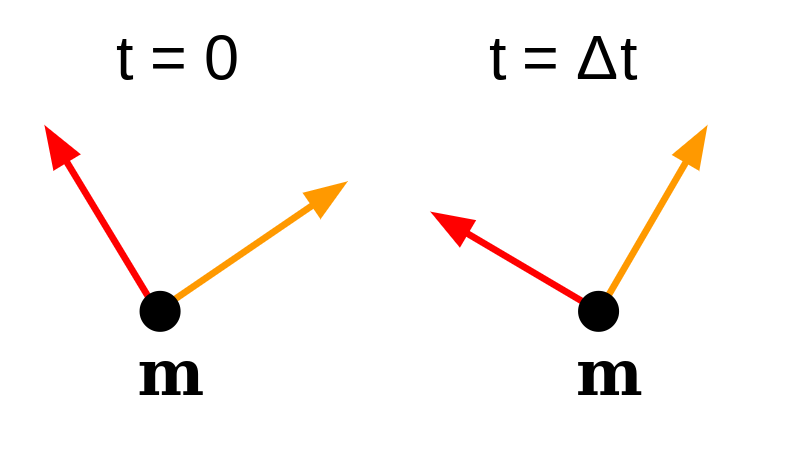
\includegraphics[width=.7\linewidth]{MillerAxes.png}   
\]

In order to view $\vec{u}$ from Miller's frame, we will have to rotate $\vec{u}$ by $-\theta(t)$. This is because in Miller's frame, the observer's world rotates at an angular velocity of $-\omega$. At a given time $t$, Miller considers the world to have rotated by $- \omega t$, which just happens to be $-\theta (t)$. In order to 'rotate back' we apply a 2x2 rotation matrix $Rot(-\theta)$ to $\vec{u}$.Thus, the path that Miller sees the ball take is given by:
\begin{equation}
\begin{split}
        \vec{u}_m & = Rot(-\theta)\vec{u} \\
        &= \langle (x_0 - \omega t y_0) cos(\theta(t)) + (y_0 + \omega t x0 )sin(\theta (t), \\
        &R+(\omega t x_0 + y_0)cos(\theta(t))+(\omega t y_0 - x_0)sin(\theta (t)) \rangle    
\end{split}
\end{equation}

\subsection*{Method 2: Arclength and Radius}
In the second method we immediately take the viewpoint of Miller. We consider the arclength between Miller and the ball to be the displacement in the x direction, while the ball's height above the ship floor to be the displacement in the y direction. We'll define the height of the ball above the ship floor as:

\[h = R - r\]

Where $r$ is the ball's distance from the center of the ship. $r$ as a function of time is given as:

\begin{equation}
\begin{split}
    r &= \lvert \vec{b} \rvert \\
    &= \sqrt{(x_0^2+y_0^2)(1+\omega^2 t^2)}
\end{split}
\end{equation}


The arclength between Miller and the ball is:
\begin{equation}
 x = \gamma R
\end{equation}

Where $\gamma$ is the angle between Miller and the ball.

\[
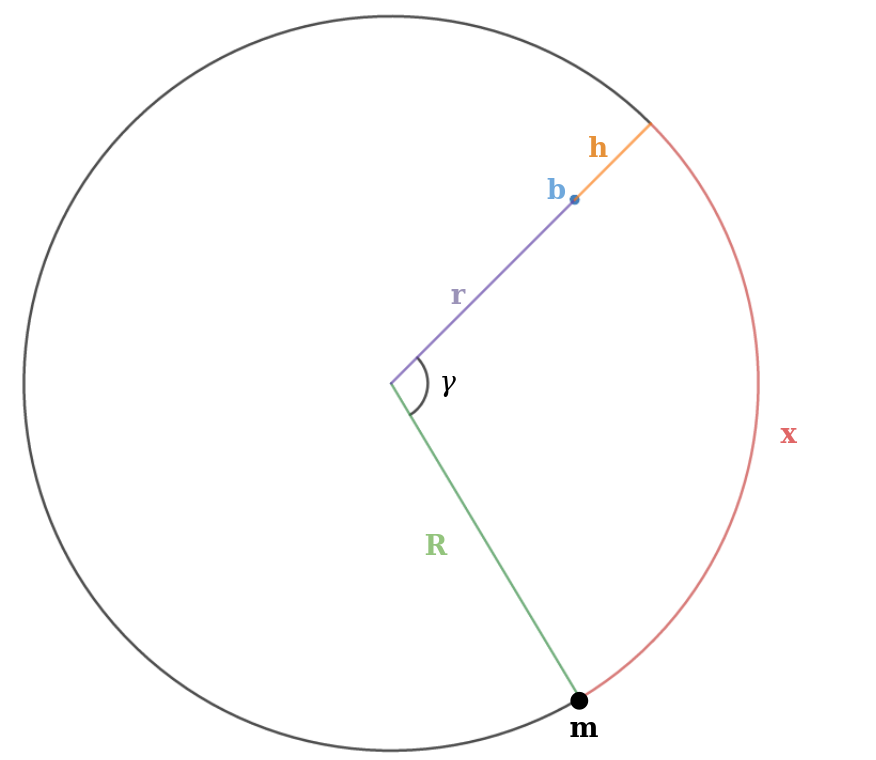
\includegraphics[natwidth = 300]{arclengthLabeled.png}
\]

$\gamma$ can easily be found by using the dot product definition:
\[\vec{m}\cdot\vec{b}= \lvert \vec{m} \rvert \lvert \vec{b} \rvert cos(\gamma)\]

And taking the $\arccos$ so that $\gamma$ is:
\begin{equation}
\gamma  = \arccos\left(\frac{\vec{m}\cdot \vec{b}}{\lvert \vec{m} \rvert \lvert \vec{b} \rvert}\right) 
 = \arccos\left (\frac{\vec{m}\cdot \vec{b}}{rR}\right)
\end{equation}

Thus the equation of motion for the ball that Miller sees is:

\begin{equation}\label{eq:uV1}
    \vec{u}_{arc} = \langle R cos(\gamma), h \rangle
\end{equation}

\subsection*{Comparison of Methods 1 and 2 to Real Gravity}

Now that we've derived the equations of motion that a ball would take
if dropped from the ship, we can compare their height as a function of
time to the height of a ball if dropped on a planet where gravity is
(approximately) constant. Our end goal is to determine what kind of
situations give realistic gravity from Miller's point of view. The $x$
components for each method are both non-zero as a function of time,
which does not line up (pun intended) with a ball dropped on
Earth. While this is important, we will not analyze the $x$ component
until the next section where we discuss projectile motion.

The height of a ball dropped on a planet with gravity $g$ with a starting height of $h_0$ is given by:
\begin{equation}
    h(t)=\frac{1}{2}gt^2 +h_0
\end{equation}

Whereas the height of a ball from the ship as a function of time given the rotation of frames method $h_{rot}(t)$ and the arclength method $h_{arc}(t)$ is given by:

\begin{equation}
    h_{rot}(t) = R+(\omega t x_0 + y_0)cos(\theta(t))+(\omega t y_0 - x_0)sin(\theta (t))
\end{equation}

\begin{equation}
    h_{arc}(t) = R - \sqrt{(x_0^2+y_0^2)(1+\omega^2 t^2)} \\
\end{equation}

In order to compare $h_{arc}(t)$ and $h_{rot}(t)$ to $h(t)$, we need to find the ship's simulated gravity for the ship's given $\omega$ and $R$. Then we will do a Taylor series expansion of $h_{arc}(t)$ and $h_{rot}(t)$ and see how the expansion terms compare to $h(t)$. We should expect the quadratic terms of the expansion to be $\frac{1}{2}gt^2$.

We will consider the gravity of the ship: $g_{ship}$  to be the acceleration that Miller feels at his feet while standing stationary. This is can be found by taking the second derivative of Miller's position with respect to time:
\begin{equation}
\begin{split}
     g_{ship}&=\lvert\vec{m}''(t)\rvert \\
     &= \frac{d^2}{dt^2}R\lvert \langle sin(\theta(t),-cos(\theta(t)\rangle \rvert \\
     &=R \omega^2
\end{split}
\end{equation}

To simplify the expansion, we assume that  $\phi$ is zero and the ball starts at $\langle x_0,y_0\rangle$ from the center of the ship. Doing a Taylor series expansion on $h_{rot}(t)$ and $h_{arc}(t)$ (with \textsl{Mathematica}) yields:
\begin{equation}
\begin{split}
     h_{rot}(t) &\approx (R+y_0)+\frac{1}{2}\omega^2 y_0 t^2 - \frac{1}{3}\omega^3 x_0 t^3 -\frac{1}{8}\omega^4 y_0 t^4... \\
     &\approx (r_0)+\frac{1}{2}\omega^2 y_0 t^2 - \frac{1}{3}\omega^3 x_0 t^3 -\frac{1}{8}\omega^4 y_0 t^4...
\end{split}
\end{equation}

\begin{equation}
 h_{arc}(t) \approx h_0 -\frac{1}{2}\omega^2 r_0 t^2 + \frac{1}{8}\omega^4 r_0 t^4 ...
\end{equation}

From the Taylor series expansion above, we can see that $h_{rot}(t)$
and $h_{arc}(t)$ are extremely similar (identical up to the 4th order
assuming $x_0$ is zero) since $g_{ship} = R \omega^2$ and $R+y_0 =
h_0$. This makes sense, as the rotation method and arclength method
only really begin to differ when $\theta(t)$ becomes large. However,
by the time $\theta(t)$ actually becomes large, the ball has long
since hit the grown of the ship. While both methods are fine
approaches to artificial gravity, we will exclusively use $h_{rot}(t)$
when comparing artificial gravity to planetary gravity. This is
because the rotation method is computationally simple (does not
require arcCosine) and comparing $h_{rot}(t)$ and $h_{arc}(t)$ along
side $h(t)$ is fruitless, as $h_{rot}(t)$ and $h_{arc}(t)$ will appear
identical when compared to the second order differences between
artificial and planetary gravity. From now on we will define
artificial gravity as:

\begin{equation}\label{eq:approxGravHeight}
\begin{split}
    h(t)_{approx} &= h(t)_{rot} \\
    &=R+(\omega t x_0 + y_0)cos(\theta(t))+(\omega t y_0 - x_0)sin(\theta (t))
\end{split}
\end{equation}

From the Taylor series expansion We also find that $h_{approx}(t)$ is approximate to real gravity when $r_0 \approx R$! Assuming Miller drops objects (such as pouring water) from eye level, we can now investigate what is "good" artificial gravity. In particular we want to investigate a `Just Noticeable Difference' for objects poured over a distance of 1 meter. According to Weber's law

Making the substitution  and $x_0 =0$ yields an identical 0th and 1st order terms to both $h_{rot}(t)$ and $h_{arc}(t)$. $h_{rot}(t)$ and $h_{arc}(t)$ differ at the 3rd order term for non-zero , but since $x_0$ is zero,  and a near identical 0th and first order term for  when $r_0 \approx R$! 


\subsection*{Method 1: Applied to Projectile motion}
Thus far we have assumed that all objects dropped in artificial
gravity are initially at rest. This works well to simply describe what
Miller sees when pouring a drink in artificial gravity. However we can
explore a rich set of scenarios and situations by deriving the
equations of motion for a drink poured with \textit{initial
  velocity}. In this section we will derive the general equations of
motion for a projectile as seen in Miller's frame using the method of
rotating frames. We will no longer consider the arc length method
because the method requires the use of the arcCosine function (which
is unnecessarily complex).


Miller's position on the ship is still given by equation
\ref{eq:MillerPosition} on page \pageref{eq:MillerPosition}:

\[\vec{m} = R\langle sin(\theta (t) ), - cos (\theta (t) ) \rangle\]

The only change in derivation will be to add an initial velocity term,
$\vec{v}_{init}$ to the position function for the ball in equation
\ref{eq:BallV1} so that way the ball now has the position function:

\begin{equation}\label{eq:BallProjectile}
\begin{split}
     \vec{b}_{projectile} &= \langle x_0 - y_0 \omega t, y_0 + x_0 \omega t \rangle + \vec{v}_{init}t \\ 
     &\textnormal{where } \vec{v}_{init} = \langle v_{y0},v_{x0} \rangle
\end{split}
\end{equation}

Much of the same machinery used in the initial derivation in Method 1
can be used when considering projectile motion. Now it is just a
matter of substituting $\vec{b}$ with $\vec{b}_{projectile}$. Equation
\ref{eq:uV1} on page \pageref{eq:uV1} can now be rewritten as:

\begin{equation}
    \vec{p} = \vec{v}_{projectile} - \vec{m}
\end{equation}

Where $\vec{p}$ is the vector going from Miller to the projectile ball
as seen from the onlooker outside the spaceship. Finally we apply a
rotation matrix $Rot(-\theta(t))$ to $\vec{p}$ to obtain the path of
the projectile ball as seen in Miller's frame.

\begin{equation}\label{eq:ProjectileMillerFrame}
\begin{split}
    \vec{p}_m &= Rot(-\theta(t))\vec{p} \\
    &= \langle (x_0 + t(v_{x0} - \omega y_0)) cos(\theta(t)) + (y_0 +t(v_{y0} + \omega x_0) sin(\theta(t)),\\
    & cos(\theta(t)) (R cos(\theta(t)) + y_0 + t(v_{y0} + \omega x_0)) \\
    &+ sin(\theta(t))(R sin(\theta(t)) + t(\omega y_0 - v_{x0})-x_0) \rangle
\end{split}
\end{equation}

There is one subtlety that we must hit on before continuing. When
dealing with projectile motion, the ball can have tangential
velocity. Initially we defined tangential velocity to generally be
$\omega r$, which was then used to define gravity as $g = \omega^2 r$.
However with the addition of some tangential velocity $v_{tang}$ the
gravity for an object on the space ship with a given position and
velocity is:
\begin{equation}\label{eq:TangentGravity}
\begin{split}
    g_{tang} = \frac{(\omega R + v_tang)^2}{R}
\end{split}
\end{equation}

\hrulefill %This is just to know where your work ends and my prior work begins

Is depiction accurate? To approximate the path the drink will take
from the perspective of Miller, we first have to see how Ceres, and
therefore Miller, is moving. Afterwards, we can find the path of the
drink, and then subtract its position function from Miller's position
function to find the drink's path in his point of view. Miller's
position function can be modeled by the parametric equation of a
circle, \vec{p}, with a radius of $R$ and angular velocity $\omega$.

\[
\vec{p}(t) = \langle R\cos(\omega t),R \sin(\omega t)\rangle
\]

%Ceres' angular velocity can be found using the centripetal acceleration equation, $a = v^2 /r$, and when solved for velocity $v$, is $v = \sqrt{aR}$. From this, we find angular velocity $\omega = v/R = \sqrt{aR}/R$, meaning that on the Ceres, for its artificial gravity $a$ created within it, and its radius $R$, it will have an angular velocity of $\sqrt{aR}/R$, and will complete a full rotation in $\frac{2\pi}{\sqrt{aR}/R}$ seconds.%

To find $\omega$, we will need to take the second derivative of $\vec{p}(t)$, $\vec{p}''(t)$, which will describe Miller's centripetal acceleration.

\[
\vec{p}''(t) = \langle -\omega^2 R \cos(\omega t), - \omega^2 R \sin(\omega t)\rangle
\]

We can then find the magnitude of the acceleration with respect to $\omega$ using the Pythagorean Theorem, $a^2 = x^2 + y^2$. Using the $x$ and $y$ values of $\vec{p}''(t)$ as well as the fact that the acceleration is $0.3g$, we have

\begin{align*}
    a^2 &= x^2 + y^2 \\
    a &= \sqrt{x^2 + y^2} \\
    &= \sqrt{(-\omega^2 R cos(\omega t))^2 + (- \omega^2 R sin(\omega t))^2} \\
    &= \sqrt{\omega^4 R^2 (\sin^2(\omega t) + \cos^2(\omega t))} \\
    &= \sqrt{\omega^4 R^2} \\
    &= \omega^2 R
    \end{align*}
    So we may write
\begin{align*}
    \omega^2 &= a / R\\
    \omega &= \sqrt{a/R}
\end{align*}

Now that we know that $\omega = \sqrt{a/R}$, we can use our knowledge
that Ceres will complete one complete rotation in
$\frac{2\pi}{\omega}$ seconds and the fact that linear velocity $v$ is
related to $\omega$ through $v = \omega R$ to find the position
function of the drink.

The drink will be poured a certain distance from the outside of Ceres,
so it will have a smaller radius, \(r\). Since this drink is no longer
influenced by Ceres' angular velocity after being poured, it will
travel tangentially from Ceres' surface at a linear velocity of \(v =
\omega r\). Using this information, and assuming the drink is poured
at $t = 0$, we have the position function of the drink, $\vec{b}(t)$,
as

\[
\vec{b}(t) = \langle r, \sqrt{\frac{a}{R}}rt\rangle
\]

Bringing it together, to find the path the drink takes from the
perspective of the person, we have to take the position function of
the drink, \vec{b}, and subtract it by the position function of the
person, \vec{p}, to get the net distance, \vec{d}(t).

\[
\vec{d}(t) = \vec{b}(t) - \vec{p}(t) = \langle r - R\cos(\sqrt{\frac{a}{R}} t), \sqrt{\frac{a}{R}}rt - R \sin(\sqrt{\frac{a}{R}} t)\rangle
\]

$\vec{n}(t)$ will track the path of the drink until it crosses the
y-axis, at which point it would be equivalent to hitting the floor of
Ceres. Plugging in the actual values of Ceres, and estimating the
drink to be poured $0.25$m above the cup, we have

\[
\vec{d}(t) = 
\begin{bmatrix}
(473000 - 0.25) - 473000\cos(\sqrt{\frac{0.3\cdot9.8}{473000}}t)\\ \sqrt{\frac{0.3\cdot9.8}{473000}}(473000 - 0.25)t - 473000 \sin(\sqrt{\frac{0.3\cdot9.8}{473000}}t)
\end{bmatrix}
\]

Finding when the x-component of $\vec{d}(t) = 0$, we find that $t =
\frac{\cos^{-1}(r/R)}{\omega} = 0.41239$ seconds, in the case given
above. solving for the y-component at $t=0.41239$, we find $y = -1.713
\cdot 10^{-4}$, meaning that casually pouring a drink would only shift
the stream less than a fifth of a millimeter from a similar pour on
Earth, following a path that resembles the beginning of a cycloid.

These effects can be magnified at greater distances. For example, if
something dropped from 10 meters, it would land about 4 centimeters
off from its Earth landing position, and from 100 meters, it would be
about 1.4 meters off. Whatever the case, the path of any falling
object, be it a drink or Miller's hat, does not resemble the path made
in The Expanse.

\section{Explosions}

In Episode 1, the \textit{Canterbury} is destroyed. 
The \textit{Knight} is then damaged by the wreckage. 
Is this realistic?

The wreckage can be modeled with the vector field:
\[
\vec{F}(x,y,z) = \frac{\vec{x}}{4\pi|\vec{x}|^3}
\]
where $\vec{x} = \langle x,y,z\rangle$

I believe the \textit{Canterbury} is $26000$ from the \textit{Knight}

Based on:

\texttt{https://www.youtube.com/watch?v=qX8TlGCsllM}

It looks like the \textit{Canterbury} is $1000$m long and $250$ m wide. 

The


\section{Cererian Gravity}

Ceres, a dwarf planet in the asteroid belt, has been spun up by Tycho Manufacturing to have a gravitational force of $0.3$g. How fast would Ceres need to spin?

For any large rotating body, its gravity pulls objects toward its center, while the rotation of it counteracts gravity, pushing objects away. If the centrifugal force of the object is greater than its gravity, objects on the surface, and the surface itself, would fly off, tangent to the surface of the planet. To verify whether Ceres can maintain an internal artificial gravity of 0.3g, we can see if Cererian gravity is greater than the artificial gravity or note (Side note: If the artificial gravity was equal to the real gravity, anything on its surface would be weightless, as all of gravity is canceled out by the centrifugal force). Cererian gravity can be found though the Newton's Law of Universal Gravitation,
\[
g=\frac{GM}{R^2}
\]
where \(G=6.67*10^{-11}\) is the gravitational constant, \(M\) is the mass of the object, and \(R\) is the radius of the object. For Ceres, \(M=9.4*10^{20}\) and \(R=4.73*10^5\), so
\[
g_{Ceres}=\frac{6.67*10^{-11}\cdot 9.4\cdot 10^{20}}{(4.73\cdot10^5)^2}=0.28\frac{m}{s^2}
\]

Since the gravitation of Ceres, $0.28 \frac{m}{s^2}$, is smaller than the centrifugal force, $0.3g$, Ceres wouldn't be able to withstand being spun up to 0.3g without losing a large part of its mass.

Knowing that $a_{centrifugal} = g$ to maintain a stable artificial gravity, many more questions arise. Is there a better candidate to spin up to achieve 0.3g? How big would Ceres look with missing mass, and how strong would the artificial gravity be? We'll take these questions one at a time.

\subsection{A Better Candidate}
In order to spin a planet so its artificial gravity is 0.3g, we need a planet that has a regular gravity over or equal to 0.3g. The closest match? Mars, with \(g_{Mars} = 0.376g\), but with the MCR already claiming the planet, the next best match is Mercury, with a very similar gravity of 0.37g.

\subsection{Ceres-ly Smaller}
Suppose Tycho followed through with spinning up Ceres to the speed necessary for 0.3g, even though it would shed a significant amount of mass. How big would this new Ceres look, and what would the artificial gravity be like inside of it?

First, we need to find the velocity of Ceres at its equator, and by manipulating \(a = \frac{v^2}{R}\), we get \(v = \sqrt{aR}= \sqrt{0.3g * 4.73 * 10^5} = 1179\frac{m}{s}\). We also know that \(\omega = \frac{v}{R} = \frac{1179}{4.73*10^5} = 0.00249\frac{rad}{s}\). Using \(v=\omega  r\) and \(a_{centripetal} = g = \frac{v^2}{r} = \frac{GM}{r^2}\), we now have 
\[
\frac{(\omega r)^2}{r} = \frac{G M}{r^2}\quad
\Leftrightarrow \quad r = \sqrt[3]{\frac{GM}{\omega}},
\]
giving us the radius of the new Ceres, which is 
\[
\sqrt[3]{
\frac{6.67*10^{-11}*9.4*10^{20}}{0.00249^2}
} = 29316m.
\]
For perspective, that's similar to something the size of a car tire disintegrating into something the size of a quarter.

Next, we need to find the mass of the smaller Ceres. We'll assume that Ceres is round and has uniform density. Given that density \(\rho = \frac{M_{old}}{V_{old}}\), where \(V=\frac{4}{3}\pi r^3\) is the volume of a sphere, we can find the new mass as 
\begin{align*}
    M_{new} &= \rho V_{new}\\
    &= \frac{M_{old}}{\frac{4}{3}\pi r_{old}^3}\cdot \frac{4\pi r_{new}^3}{3} \\
    &= \frac{M_{old}r_{new}^3}{r_{old}^3} \\
    &= \frac{9.4\cdot10^{20} \cdot 29316^3}{(4.73\cdot 10^5)^3} \\
    &= 2.24\cdot10^{17}kg.
\end{align*}

Finally, to find the maximum artificial gravity of the smaller Ceres, we just need to find the surface gravity of it, which would be \(\frac{GM_{new}}{r_{new}^2}=\frac{6.67*10^{-11}*2.24*10^{17}}{(29316)^2} = 0.017\frac{m}{s^2} = 0.0018g\), falling short of the 0.3g goal by quite a large amount.









\section{More Questions \& Thoughts}
\begin{enumerate}
    \item How do the magnetic boots work? Can you "turn off" magnetism in boots?
    \subitem How would it feel? Additional manipulation of the magnetic field?
    
    \item Season 1, Episode 7. Are the vertical windmills in the back of Holden's house more efficient than traditional wind turbines?
    
    \item Shed's blood in 0g, would it actually congregate into a ball?
    \item How quickly would air evacuate with a hole in the wall?
    \subitem How long until Nauvoo lost all air?
    \item How strong was the radiation that hit Miller and Holden, based on symptoms and time exposed?
    \item Realistic travel times? From Tachi/Rocinante to Tycho, Tycho to Anubis to Eros, Phoebe to Eros? Earth to Phoebe?
    \subitem How much fuel would be needed?
    \item Spread of disease in the second season?
    \item How much power would it take to blow up Phoebe/Deimos?
    \item Belter bones + falling from switch of 0g to 0.3g. Anything broken?
    \item Nikil fell down out of the airlock. Shouldn't he have fallen sideways?
    \item What would be needed for Martians to train at 1g? On a spaceship? Wouldn't that crush Martian bones like Belters in 1g?
    \subitem Possibly a ship travelling in circles? how big is that circle?
    \item What's the circumference of the Belt?
    \item How many lightseconds is the Belt from Earth/Mars, at closest and farthest distances? (For communication delay purposes)
    \item How long would the Nauvoo trip take? Where are they going?
    \item What's the max velocity of a trip of distance x? (given it's 0.3g acceleration)
    \item The Nauvoo-Eros collision course for the Sun is inaccurate.
    \subitem Given that it's accurate, how fast would the Nauvoo be when it would it Eros?
    \subitem how long would it take to plummet into the Sun?
    \item How strong are the suit thrusters? How many are there? Waste of matter?
    \item How heavy can something be in 0g? (Like Miller's bomb?)
    \item How fast was the Marasmus debris hitting Miller?
    \item How much force needed to more Eros 1 radius?
    \subitem What is the radius of Eros?
    \item What's the population of Eros?
    \subitem Is the disease spread time realistic? How long should it take?
    \item How fast is Eros moving?
    \item Power of Miller's nuke?
    \item Are face lights in a suit actually effective, or just cinematic necessities?
    \item Would it be hard to cool electronics in a vacuum?
    \item Energy required to get out of the Hill radius?
    \item Fuel needed to travel between places? time? min/max?
    \item Time needed to travel from Mars to Phoebe? from Earth? What positioning would be needed to get there at the same time?
    \item Ceres population? How much water needed to keep it alive?
    \item How much water/air/acres of land for food needed for one human for one day?
    \item How much water could the Canterbury hold? How big is the Cant/Roci?
    \item Are trees on Ceres efficient? (use water, give oxygen)
    \item Escape velocity of moon? Mars? Belt asteroids?
    \item 13 minute delay in ep 5, how far away is Roci and Eros from Earth?
    \item Would the Nauvoo take that long to zoom by Eros?
    \item Could you throw a punch in 0.3g? 0g?
    \item How much more dense would Mars need to be to hold an Earth-like atmosphere?
    \item Given density of matter in space, how many holes should the Nauvoo have by the end of its trip? Is that realistic for survival?
    \item Surface area of Nauvoo?
    \item Martian population?
    \item Force needed to break a rock?
    \item g's needed to kill a human? Knock them out?
    \item How fast was Bizi Betiko going to get killed?
    
    \item Do scoped earth guns work on mars?scopes have equally spaced ridge lines that allow the shooter to accpunt for a bullet's drop. Would these scoped guns work on mars, where the gravity is less than that of earth's?
    \item Continuation of question above...how would a bullet behave on a ship with artificial gravity (generated by centrifugal force). How would you build a scope for a gun in such a case?
    \item Turn on a dime in space? In The Expance, small crafts rotate with ease. How do real space craft manage to rotate?
    \item How do you brew coffee in zero G?
    \item what is the accelertion of the ship at 28:48? assume the camera is not acceleratin and that [part to be determined] is approximately [size to be determined].
    \item Crew members use magnetic shoes in zero G environments. What is the force on their ankles? How would that force change if they used knee length rigid magnetic boots instead?
    \item In episode 1 at 40:46, the low gravity environment is made apparent by a bird that seems to float. can you calculate the acceleration of the bird as it drops? Are there any split second counter examples of objects falling, such that their velocity is incomsistent with the bird falling?
    
\end{enumerate}
if the



\end{document}



